% ==============================================================================
% LAB 118
% GRUNDLÄGGNADE MÄTINSTUMENT
% --------------------------
% Last updated <2015-02-18> 
%
% Author:
% Jonas Sjöberg     <tel12jsg@student.hig.se>
% Oscar Wallberg    <tco13owg@student.hig.se>
% 
% License:
% Creative Commons Attribution-NonCommercial-ShareAlike 4.0 International
% See LICENSE.md for full licensing information.
% ==============================================================================

% ==============================================================================
% INCLUDES AND CONFIGURATION
% ==============================================================================
\documentclass[11pt,a4paper]{article}
\usepackage[utf8]{inputenc}
\usepackage{siunitx} % Provides the \SI{}{} and \si{} command for typesetting SI
\usepackage{amssymb}
\usepackage{amsmath}
\usepackage{amsfonts}
\usepackage{graphicx}
\usepackage{booktabs}
\usepackage{longtable} % Tables span across pages
\usepackage{microtype}
%\usepackage[swedish]{isodate}
\usepackage{gensymb}

\setlength\parindent{0pt} % Removes all indentation from paragraphs

% ==============================================================================
% DOCUMENT METADATA 
% ==============================================================================
\title{EE466 \\ Lab 118 \\ Grundläggande Mätinstrument}

\author{\\
  Jonas Sjöberg\\
  Högskolan i Gävle,\\
  Elektronikingenjörsprogrammet,\\
  \texttt{tel12jsg@student.hig.se}\\
  \\
  Oscar Wallberg\\
  Högskolan i Gävle,\\
  Dataingenjörsprogrammet,\\
  \texttt{tco13owg@student.hig.se}\\}

\date{}
% ==============================================================================
\begin{document}
% ==============================================================================
\maketitle

\begin{center}
\begin{tabular}{l r}
    % TODO
    Labb utförd: & DD Month Year \\
    Instruktör: & John Doe, John Doe
\end{tabular}
\end{center}

% ==============================================================================
% ABSTRACT
% ==============================================================================
\begin{abstract}
    Syftet med laborationen är att lära känna de vanligaste basinstrumenten i
    ett elektroniklaboratorium och innefattar övningar i att hantera
    oscilloskop, multimeter, nätaggregat, och funktionsgenerator.
\end{abstract}

\newpage

{
    %\hypersetup{linkcolor=black}
    \setcounter{tocdepth}{3}
    \tableofcontents
}

\newpage

% ==============================================================================
% SECTION: INTRODUKTION 
% ==============================================================================
\section{Introduktion}\label{setup}
% ==============================================================================
% TODO
Laborationen handlar om olika typer av elektronikinstrument
% ==============================================================================
% SECTION: 1.1 OSCILLOSKOPET
% ==============================================================================
\section{Oscilloskopet}\label{}
% ==============================================================================
% TODO

\subsection{Mätning av likspänning}\label{meas_dc}
% ------------------------------------------------------------------------------
% TODO

\subsection{Mätning av växelspänning}\label{meas_ac}
% ------------------------------------------------------------------------------
% TODO

% ==============================================================================
% SECTION: MULTIMETERN
% ==============================================================================
\section{Multimetern}\label{}
% ==============================================================================
Vi skall koppla upp en spänningsdelare med två motstånd enligt 
Figur~\ref{fig:2-mm-schem} och använda två multimetrar för att mäta strömmen 
\textbf{I} och spänningen \textbf{U}. Som spänningskälla använder vi 
nätaggregatet. Vi börjar med att välja ut motstånden \textbf{R1} och \textbf{R2}
och undersöka dessa.

\begin{figure}[htbp]
    \centering
        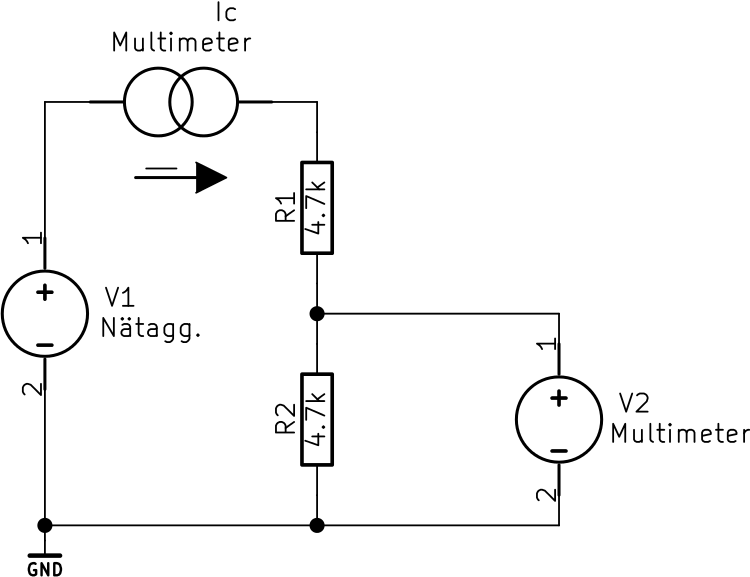
\includegraphics[scale=0.5]{kicad/2-multimeter-schema.png}
    \caption{Spänningsdelarkoppling}
    \label{fig:2-mm-schem}
\end{figure}

Tag två motstånd med olika resistansvärden i området $1-10k\Omega$.
Anslut motstånden till en multimeter med labsladdar och krokodilklämmor.
Mät upp resistanserna med multimetern och jämför med resistansvärdena som är
angivna med färgkoden på motstånden. Välj mätområde på multimetern så att
största antalet siffror (högsta noggrannhet) erhålls.

\begin{longtable}[c]{@{}lll@{}}
    \toprule\addlinespace
    $U_{}$ (V) & Beräknat värde ($\Omega$) &  Uppmätt värde ($\Omega$)
    \\\addlinespace
    \midrule\endhead
    0 & 0 & 0
    \\\addlinespace
    0 & 0 & 0
    \\\addlinespace
    0 & 0 & 0
    \\\addlinespace
    \bottomrule
    \addlinespace
    \caption{Idealfall och mätresultat}
    \label{vdivtable}
\end{longtable}




\subsection{Mätning av spänning, ström och resistans}\label{meas_multi}
% ------------------------------------------------------------------------------
% TODO

\subsection{Mätresultat}\label{TODO}
% ------------------------------------------------------------------------------
% TODO

% ==============================================================================
% SECTION: RESULTAT
% ==============================================================================
\section{Resultat}\label{setup}
% ==============================================================================
% TODO

\newpage

% ==============================================================================
% SECTION: REFERENSER
% ==============================================================================
\section{Referenser}\label{refs}
% ==============================================================================

\subsection{www}\label{interwebs}
% ------------------------------------------------------------------------------
% TODO

\subsection{Trycksaker}\label{literature} %???
% ------------------------------------------------------------------------------
% TODO

%\subsection{Källkod}\label{sourcefiles}
% ------------------------------------------------------------------------------

% ==============================================================================
\end{document}
% ==============================================================================
